\documentclass[12pt]{article}
\usepackage[english]{babel}
\usepackage[utf8x]{inputenc}
\usepackage{amsmath}
\usepackage{graphicx}
\usepackage[colorinlistoftodos]{todonotes}
\usepackage{xcolor}
\usepackage{framed}
\usepackage{tikz}
\usepackage{titletoc}
\usepackage{etoolbox}
\usepackage{lmodern}
\usepackage{hyperref}

% definition of some personal colors
\definecolor{myred}{RGB}{125,17,12}
\definecolor{myyellow}{RGB}{225,216,183}

% command for the circle for the number of part entries
\newcommand\Circle[1]{\tikz[overlay,remember picture] 
  \node[draw,circle, text width=18pt,line width=1pt] {#1};}

% patching of \tableofcontents to use sans serif font for the tile
\patchcmd{\tableofcontents}{\contentsname}{\sffamily\contentsname}{}{}
% patching of \@part to typeset the part number inside a framed box in its own line
% and to add color
\makeatletter
\patchcmd{\@part}
  {\addcontentsline{toc}{part}{\thepart\hspace{1em}#1}}
  {\addtocontents{toc}{\protect\addvspace{20pt}}
    \addcontentsline{toc}{part}{\huge{\protect\color{myyellow}%
      \setlength\fboxrule{2pt}\protect\Circle{%
        \hfil\thepart\hfil%
      }%
    }\\[2ex]\color{myred}\sffamily#1}}{}{}

%\patchcmd{\@part}
%  {\addcontentsline{toc}{part}{\thepart\hspace{1em}#1}}
%  {\addtocontents{toc}{\protect\addvspace{20pt}}
%    \addcontentsline{toc}{part}{\huge{\protect\color{myyellow}%
%      \setlength\fboxrule{2pt}\protect\fbox{\protect\parbox[c][1em][c]{1.5em}{%
%        \hfil\thepart\hfil%
%      }}%
%    }\\[2ex]\color{myred}\sffamily#1}}{}{}
\makeatother

% this is the environment used to typeset the section entries in the ToC
% it is a modification of the leftbar environment of the framed package
\renewenvironment{leftbar}
  {\def\FrameCommand{\hspace{6em}%
    {\color{myyellow}\vrule width 2pt depth 6pt}\hspace{1em}}%
    \MakeFramed{\parshape 1 0cm \dimexpr\textwidth-6em\relax\FrameRestore}\vskip2pt%
  }
 {\endMakeFramed}

% using titletoc we redefine the ToC entries for parts, chapters, sections, and subsections
\titlecontents{part}
  [0em]{\centering}
  {\contentslabel}
  {}{}
\titlecontents{section}
  [0em]{\vspace*{1.2\baselineskip}}
  {\parbox{4.5em}{%
    \hfill\Huge\sffamily\bfseries\color{myred}\thecontentspage}%
   \vspace*{-2.3\baselineskip}\leftbar\textsc{\small\thecontentslabel}\\\sffamily}
  {}{\endleftbar}
\titlecontents{subsection}
  [8.4em]
  {\sffamily\contentslabel{3em}}{}{}
  {\hspace{1.5em}\nobreak\itshape\color{myred}\contentspage}

\renewenvironment{abstract}
 {\small
  \begin{center}
  \bfseries \abstractname\vspace{-.5em}\vspace{0pt}
  \end{center}
  \list{}{
    \setlength{\leftmargin}{.5cm}%
    \setlength{\rightmargin}{\leftmargin}%
  }%
  \item\relax}
 {\endlist}

\begin{document}

\begin{titlepage}

\newcommand{\HRule}{\rule{\linewidth}{0.5mm}}

\center 
 
%----------------------------------------------------------------------------------------
%   HEADING SECTIONS
%----------------------------------------------------------------------------------------

\textsc{\LARGE Indiana University Bloomington}\\[1.5cm] 
\textsc{\Large CSCI B 565}\\[0.5cm] 
\textsc{\large Data Mining}\\[0.5cm] 

%----------------------------------------------------------------------------------------
%   TITLE SECTION
%----------------------------------------------------------------------------------------

\HRule \\[0.4cm]
{ \huge \bfseries Data Analytics for IU Bus System}\\[0.4cm] 
\HRule \\[1.5cm]
\large Group Name : RedMiners \\
 
%----------------------------------------------------------------------------------------
%   AUTHOR SECTION
%----------------------------------------------------------------------------------------

\begin{minipage}{0.4\textwidth}
\begin{flushleft} \large
\emph{Authors:}\\
\textsc{Jayasankar, Siddharth \ Nagarajan, Ganesh \ Madhavan, Sarvothaman } 
\end{flushleft}
\end{minipage}
~
\begin{minipage}{0.4\textwidth}
\begin{flushright} \large
\emph{Supervisor:} \\
\textsc{Dr. Dalkilic, Mehmet} 
\end{flushright}
\end{minipage}\\[2cm]


%----------------------------------------------------------------------------------------
%   DATE SECTION
%----------------------------------------------------------------------------------------

{\large \today}\\[2cm] 
%----------------------------------------------------------------------------------------
%   LOGO SECTION
%----------------------------------------------------------------------------------------


\includegraphics[scale=0.5]{iu_logo}\\[1cm] 
%----------------------------------------------------------------------------------------

\vfill 

\end{titlepage}


\begin{abstract}
University Bus systems are widely used for shuttling students, faculty and patrons in and out of University campuses and still remains the easiest way to reach the University Campuses. Indiana University operates its bus system under the name IU Bus and the details are available at \url{http://www.iubus.indiana.edu/campus_bus/index.html} \\ \\
This paper attempts to develop an uniform framework and processes for analyzing IU Bus data and thus along the process hopes to establish a general framework. Any such framework should be able to transform practical nuances into presentable data analytics. The areas focused in this paper consider various aspects of discussion with the key stake holders, developing glossary, developing metrics for measuring performance,data pipe lining, data visualization, Model creation and model verification.\\ \\
This project uses MySql as its preferred database for storing operational data, Neo4j graphical database for holding aggregated data, Tableau Public for visualizing the data and R for model creation and verification.
\end{abstract}

\clearpage

\tableofcontents
\clearpage

\section{Introduction}
University Bus systems are critical for shuttling students in and out of university campuses. These bus systems are not only used at Indiana University, but also at other universities like University Transit Service,University of Virginia \url{http://www.virginia.edu/parking/uts/}, The Bus, Boston University system \url{http://www.bu.edu/thebus/}. All these universities have similar kind of schedules for different terms like Spring, Fall and special trips during late nights, called $Night Owl$ in the IU System. All these services have an live tracking system which records the bus statuses, Geo-locations of buses and their stops and is presented real-time to the users.\\ \\
IU Bus system has four routes A,B,E and X and has about 52 stops including the minor and major stops. These busses are scheduled about one bus in every 15 minutes for use of its passengers. IU Bus System commits itself to keep up the time as per the schedule at \url{http://www.iubus.indiana.edu/campus_bus/bus_schedule.html}, however as with any transportation system, the bus gains or looses speed during the course of the travel. \\ \\
Thus, primary interest of this study if to understand the time difference between the schedule time and the actual time, $t_{schedule} - t_{actual}$. An model was created in Neo4j depicting the acutal bus system

\clearpage

\section{Problem Description}
\section{Constraints}
\section{Data Management}
\subsection{Source Data Model}
Text Explanation here\\
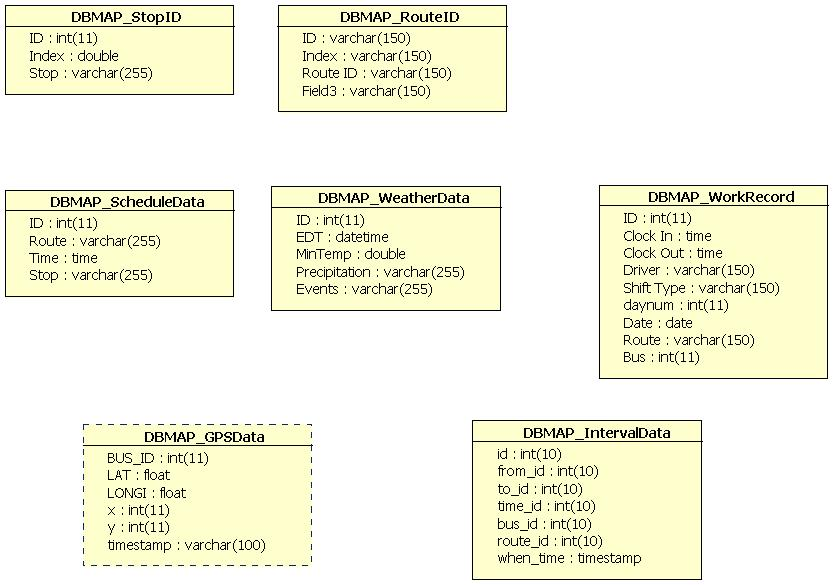
\includegraphics[scale=0.5]{resources/dbmap_access}\\[1cm] 
Text Explanation here\\
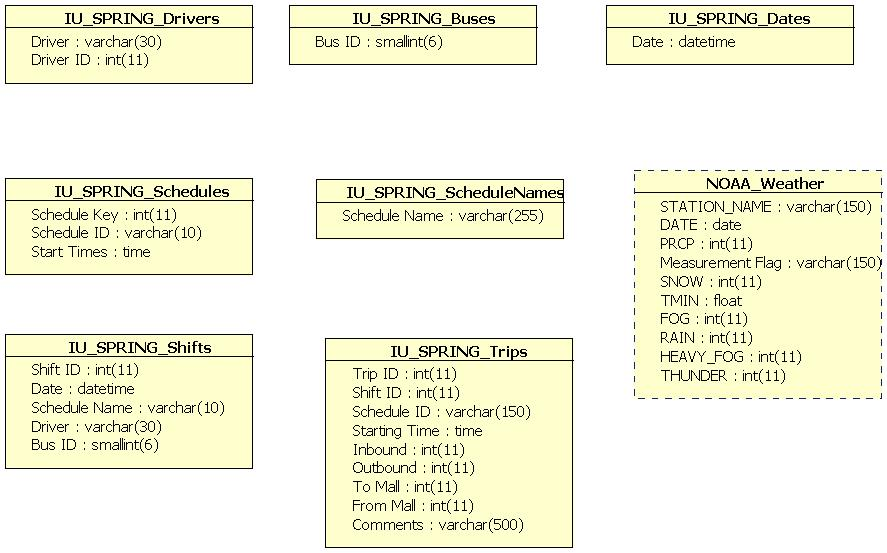
\includegraphics[scale=0.5]{resources/IU_access}\\[1cm] 
\subsection{Intermediate Model}
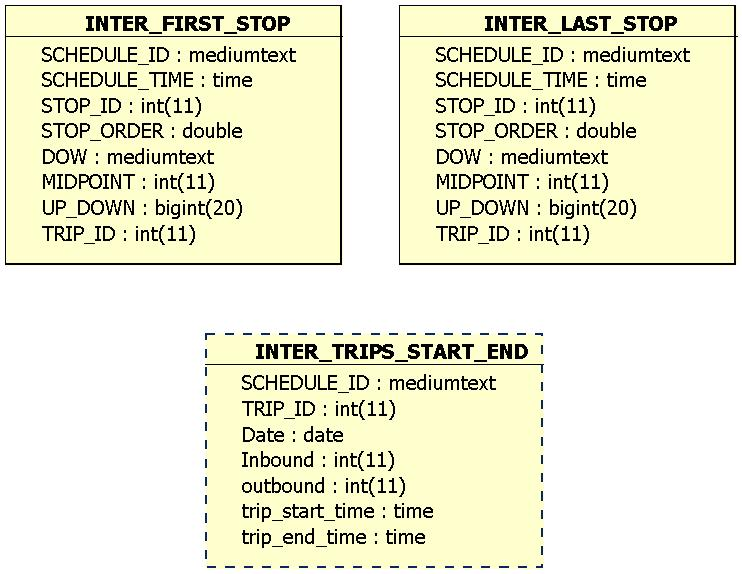
\includegraphics[scale=0.5]{resources/Inter_schedule}\\[1cm] 
Text Explanation here\\
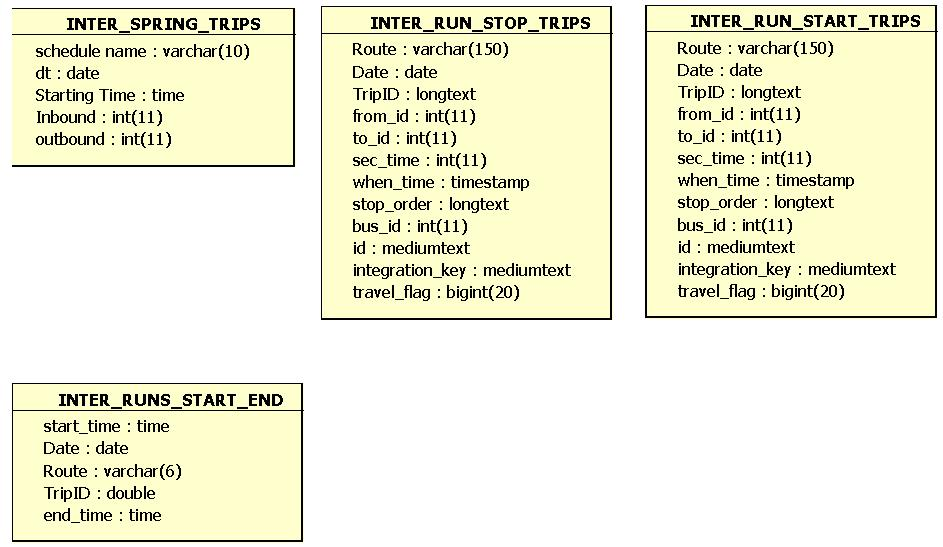
\includegraphics[scale=0.5]{resources/Inter_runs}\\[1cm] 
Text Explanation here\\
\subsection{Final Data Model}
Text Explanation here\\
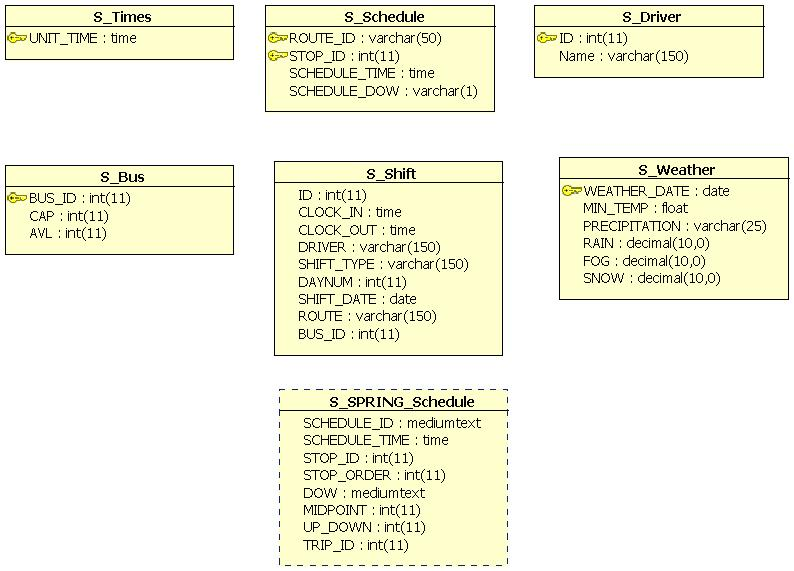
\includegraphics[scale=0.5]{resources/Source_spring}\\[1cm] 
Text Explanation here\\
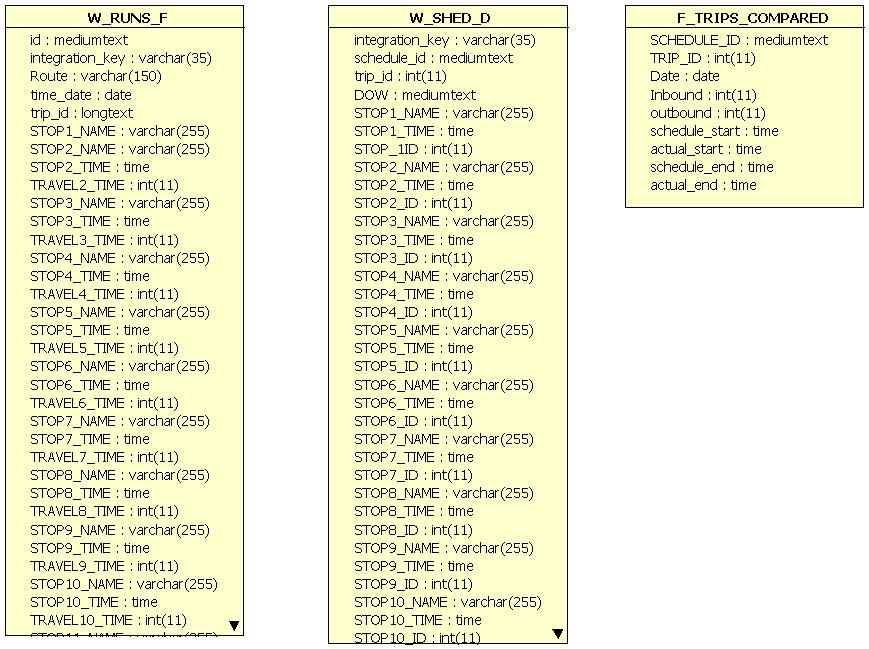
\includegraphics[scale=0.5]{resources/wh}\\[1cm] 
\subsection{Data Preparation}
Text Explanation here\\
%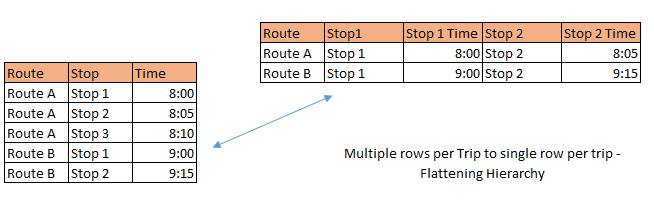
\includegraphics[scale=0.6]{resources/hierarchy}\\[1cm] 
\section{Exploratory Analysis}
Text Explanation here\\
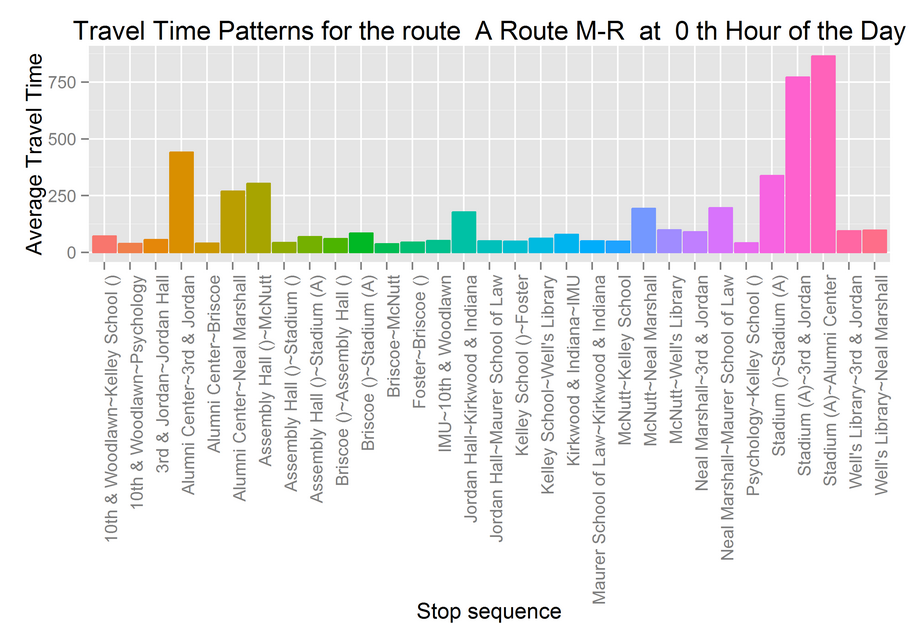
\includegraphics[scale=0.6]{resources/ggplot1}\\[1cm] 
Text Explanation here\\
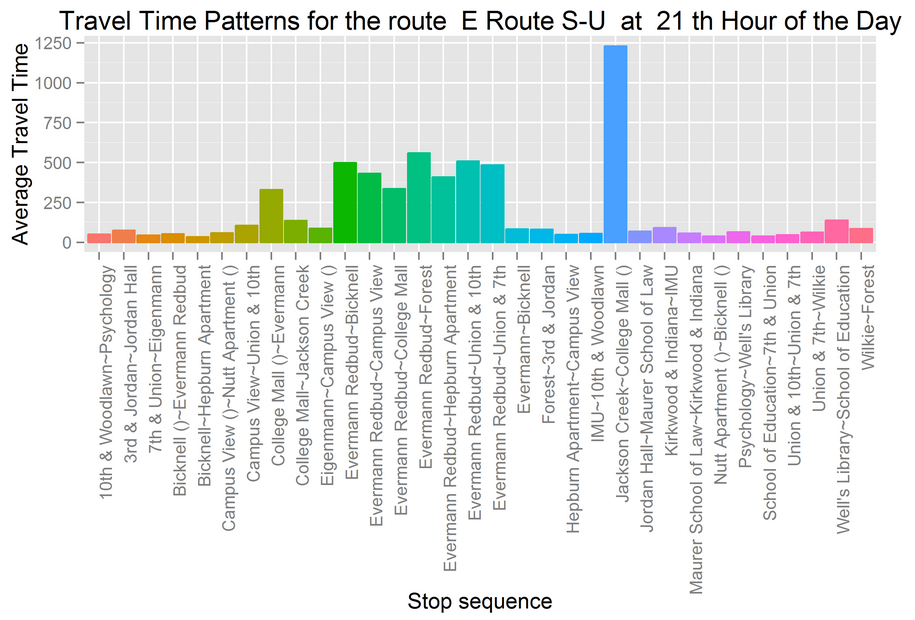
\includegraphics[scale=0.6]{resources/ggplot2}\\[1cm] 
Text Explanation here\\
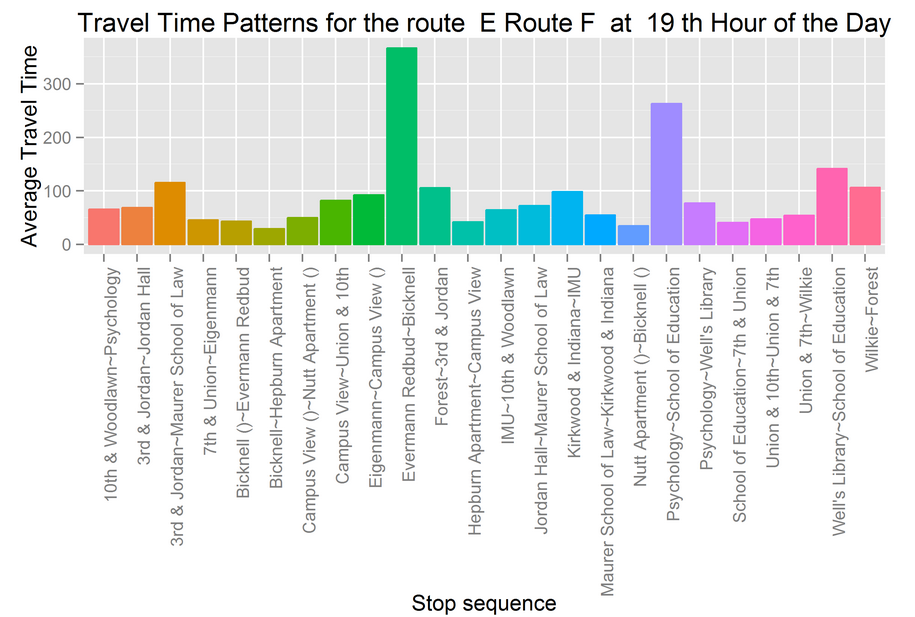
\includegraphics[scale=0.6]{resources/ggplot3}\\[1cm] 
Text Explanation here\\
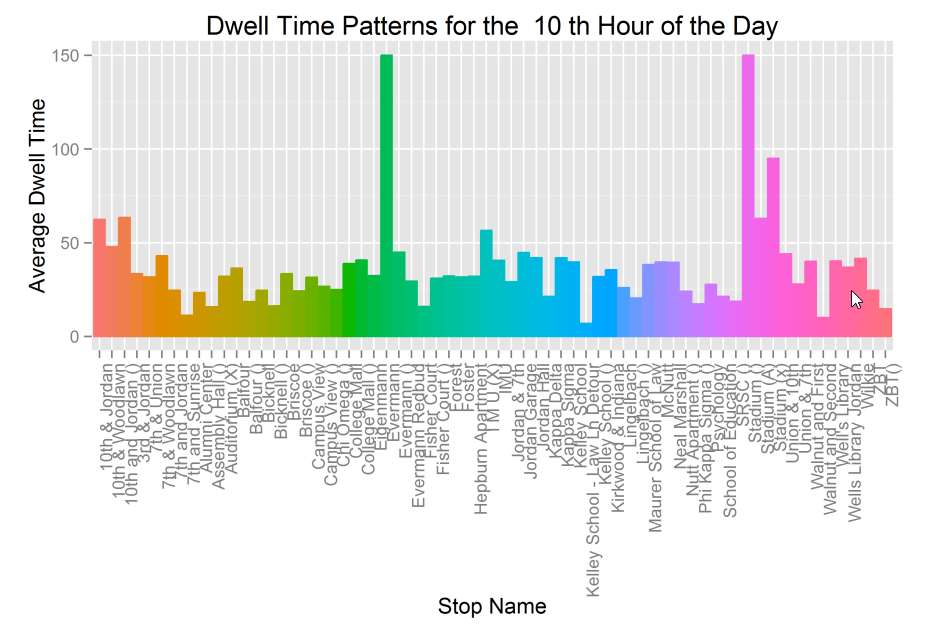
\includegraphics[scale=0.6]{resources/ggplot4}\\[1cm] 
Text Explanation here\\
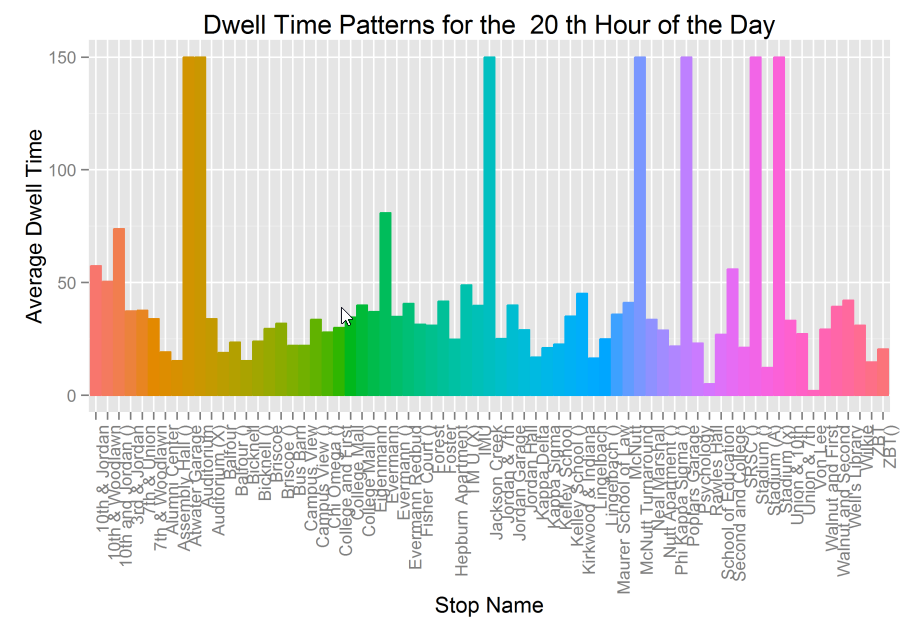
\includegraphics[scale=0.6]{resources/ggplot5}\\[1cm] 
\section{Reporting}
Text Explanation here\\
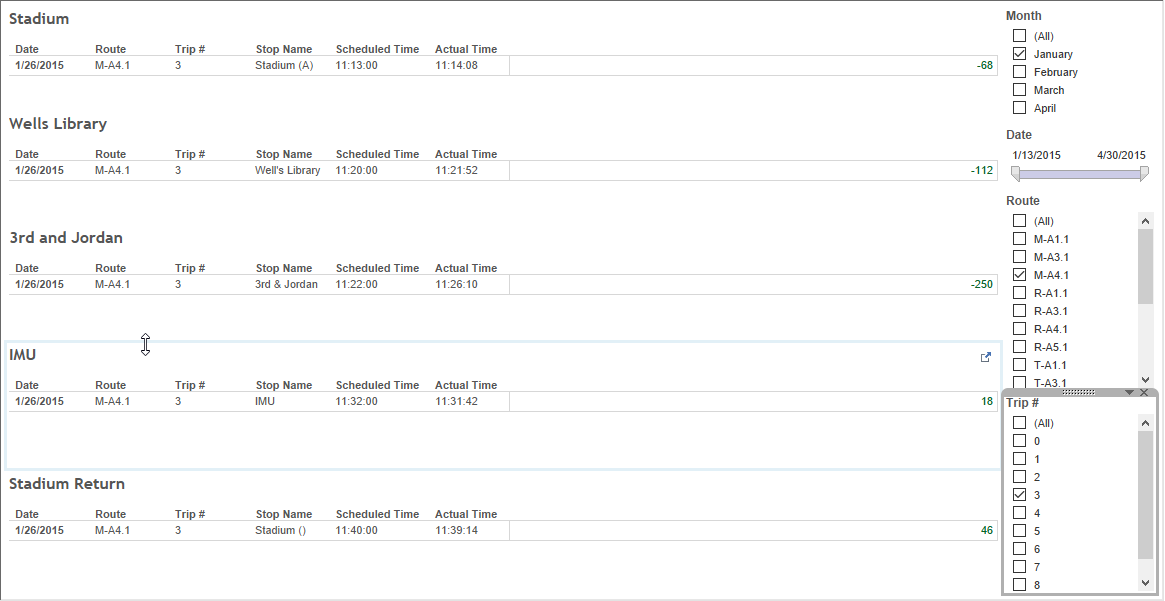
\includegraphics[scale=0.55]{resources/tableau4}\\[1cm] 
Text Explanation here\\
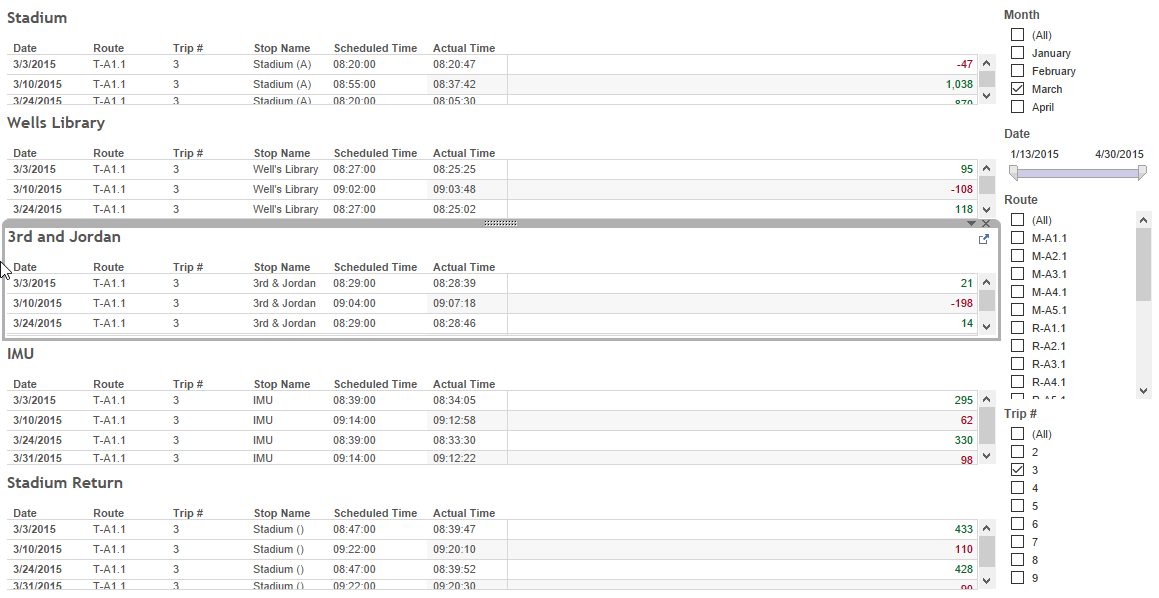
\includegraphics[scale=0.55]{resources/tableau5}\\[1cm] 
Text Explanation here\\
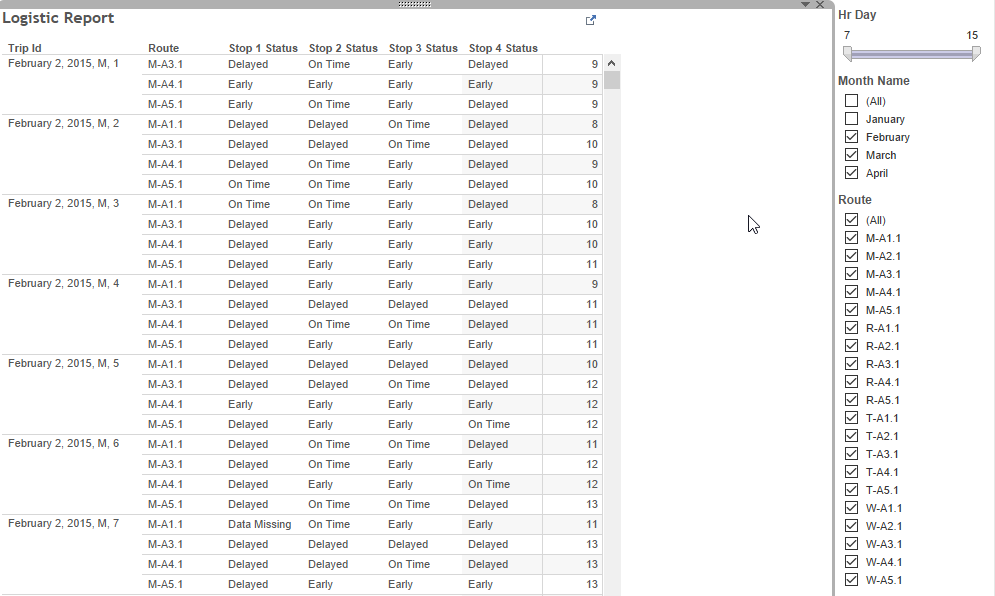
\includegraphics[scale=0.55]{resources/tableau6}\\[1cm] 
\section{Visualization}
Text Explanation here\\
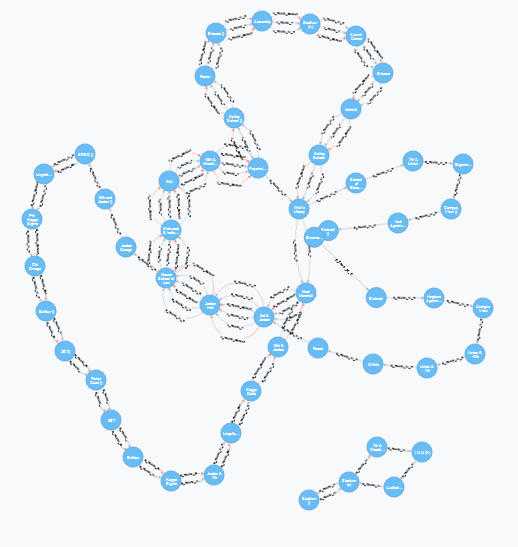
\includegraphics[scale=1]{resources/neo4j1}\\[1cm] 
Text Explanation here\\
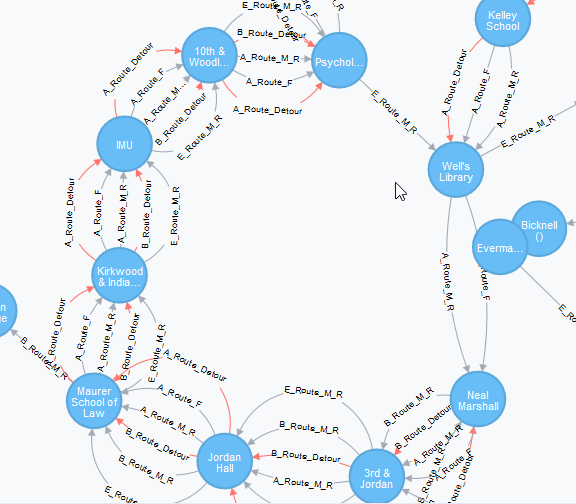
\includegraphics[scale=1]{resources/neo4j2}\\[1cm] 
Text Explanation here\\
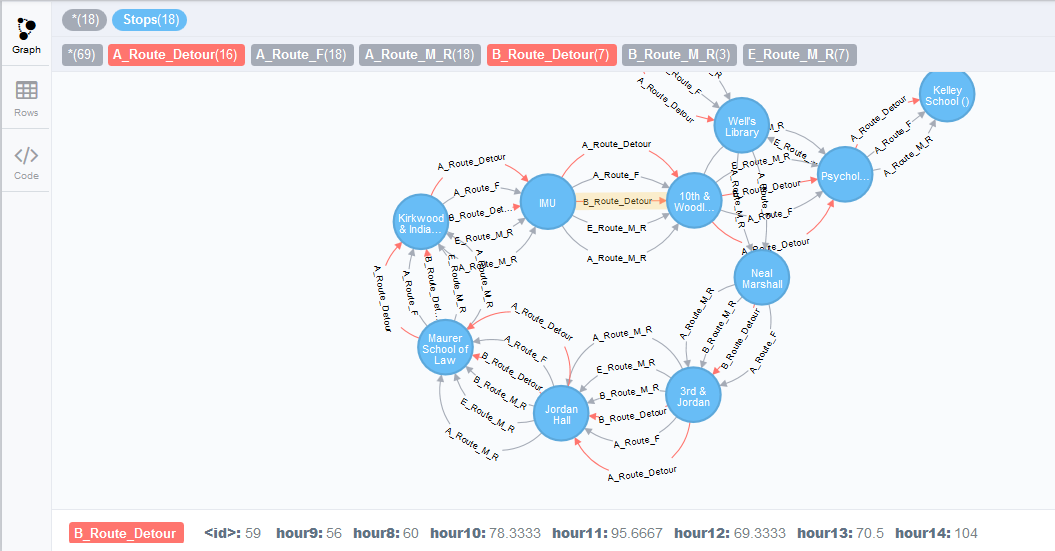
\includegraphics[scale=0.55]{resources/neo4j3}\\[1cm] 
Text Explanation here\\
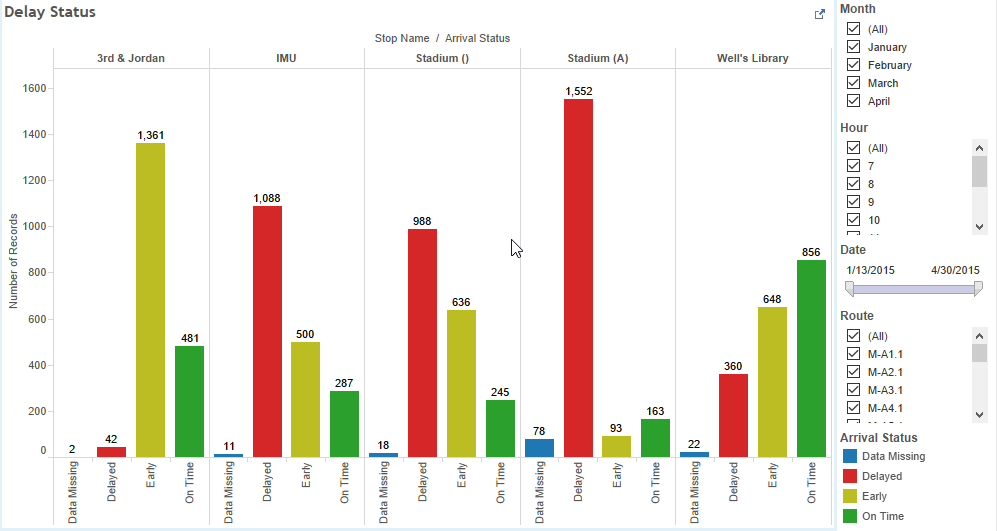
\includegraphics[scale=0.55]{resources/tableau1}\\[1cm] 
Text Explanation here\\
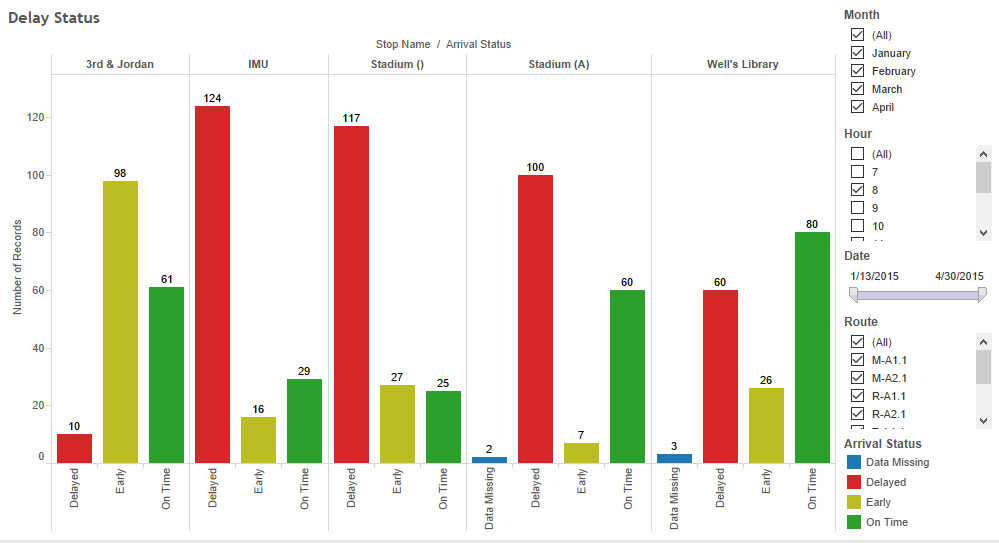
\includegraphics[scale=0.55]{resources/tableau2}\\[1cm] 
Text Explanation here\\
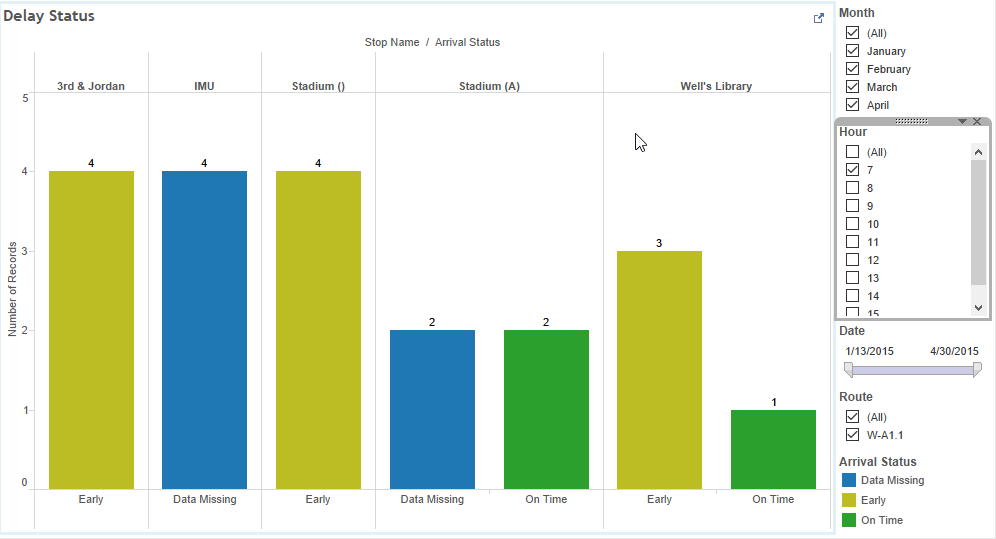
\includegraphics[scale=0.55]{resources/tableau3}\\[1cm] \section{Statistical Model}
\section{Future Work}
\section{Concluding remarks}
\section{References}
\end{document}